\documentclass[11pt]{article}
\usepackage[letterpaper, margin=1in]{geometry}
\usepackage{listings}
\usepackage{graphicx}
\usepackage{amsmath}
\usepackage{amsfonts}

\title{Homework 01}
\author{Zach Stecher}
\date{Due: 9/20/16}

\begin{document}
\lstset{language=Python}

\maketitle

\section*{Problem 1.2}
\subsection*{1.2a)}

We know that the regions represented h(x) = +1 and h(x) = -1 can be seperated by a line because h(x) = 0 seperates the two reasons, so the line that seperates the two regions is h(x) = 0.
\\

h(x) = 0 can be represented as:

\begin{equation}
	x_0w_0 + x_1w_1 + x_2w_2 = 0
\end{equation}
\\

By moving some of the equation to the other side, we end up with:

\begin{equation}
	x_2 = \frac{-w_0 - x_1w_1}{w_2}
\end{equation}

From there, if we move $-w_0$ to the end and split this side of the equation up for clarity, we get:

\begin{equation}
	x_2 = \frac{-x_1w_1}{w_2} - \frac{w_0}{w_2}
\end{equation}

So using $y = mx + b$ where $m$ is the slope and $b$ is the intersect, in terms of $w$ and $x$ the slope is $\frac{-x_1}{w_2}$ and the intersect is $\frac{-w_0}{w_2}$.
\\

\subsection*{1.2b Draw figures for cases w = [1, 2, 3] and w = -[1, 2, 3]}
\begin{figure}
	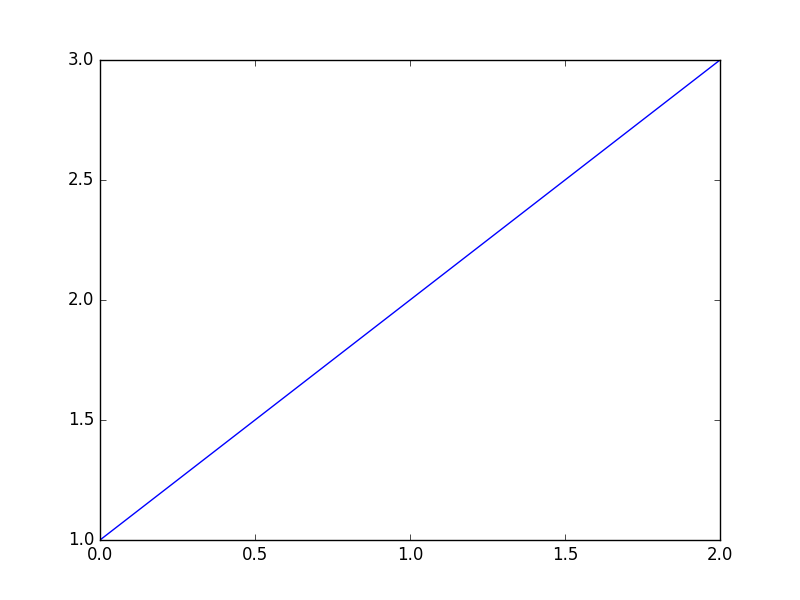
\includegraphics{12bpos.png}
	\caption{With positive weight values.}
\end{figure}

\begin{figure}
	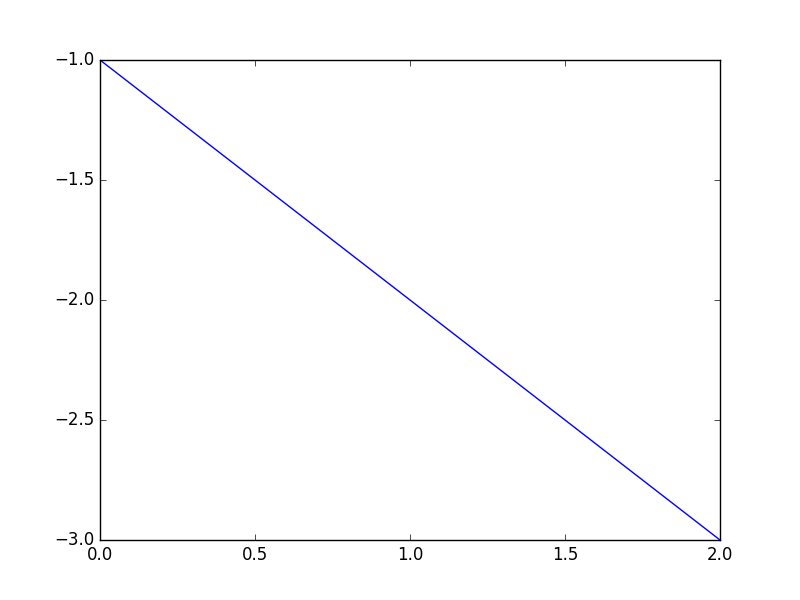
\includegraphics{12bneg.png}
	\caption{With negative weight values}.
\end{figure}
\newpage

\section*{Problem 1.4}

For all sections of problem 1.4, we used a provided base version of the Perceptron learning algorithm with small modifications.

\subsection*{1.4a}

For this section, the Perceptron was called on a deta set size 20 by the following code:

\begin{lstlisting}[frame=single]
p = Perceptron(20)
p.plot()
\end{lstlisting}

\begin{figure}[!htb]
	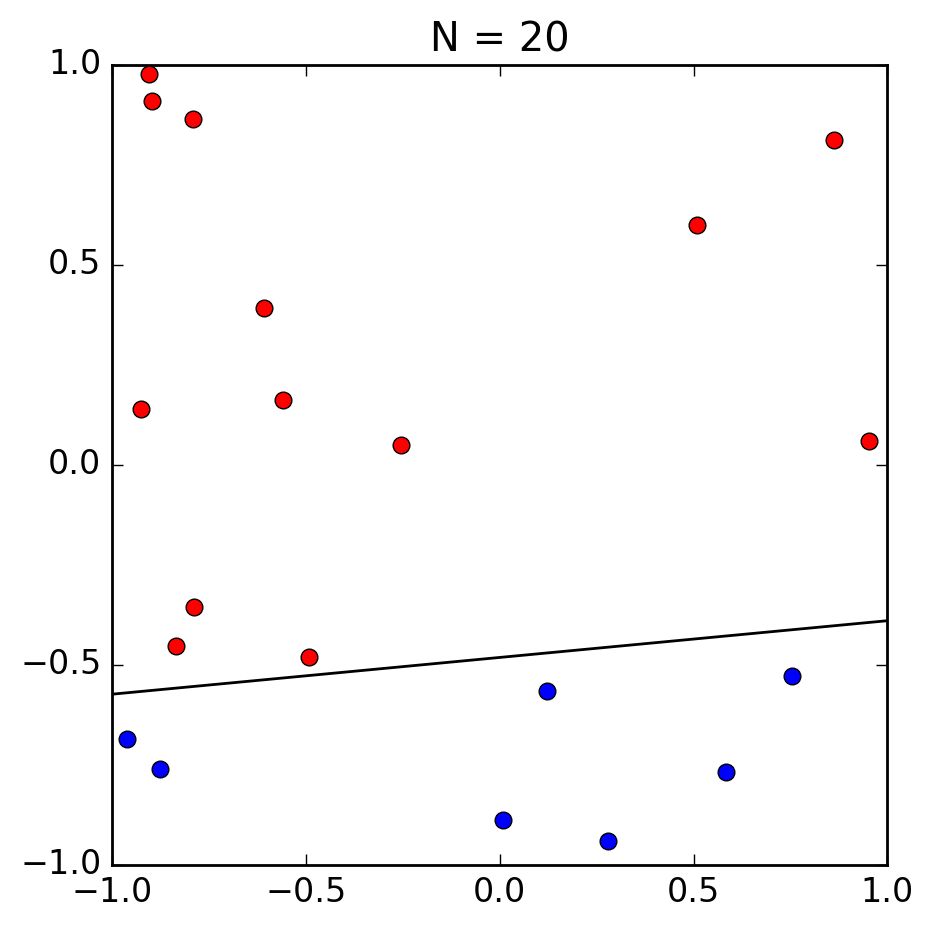
\includegraphics{14a.png}
	\caption{The final hypothesis $h(g)$.}
\end{figure}
\newpage

\subsection*{1.4b}

For this section, we ran the Perceptron algorithm again on a data set with a size of 20, taking note of the number of iterations necessary to reach $h(g)$. For this instance, we ended up with 17 iterations to reach $h(g)$.
The code was modified to save all iterations as .png files:

\begin{lstlisting}[frame=single]
p = Perceptron(20)
p.pla(save=True)
p.plot()
\end{lstlisting}

\begin{figure}[!htb]
	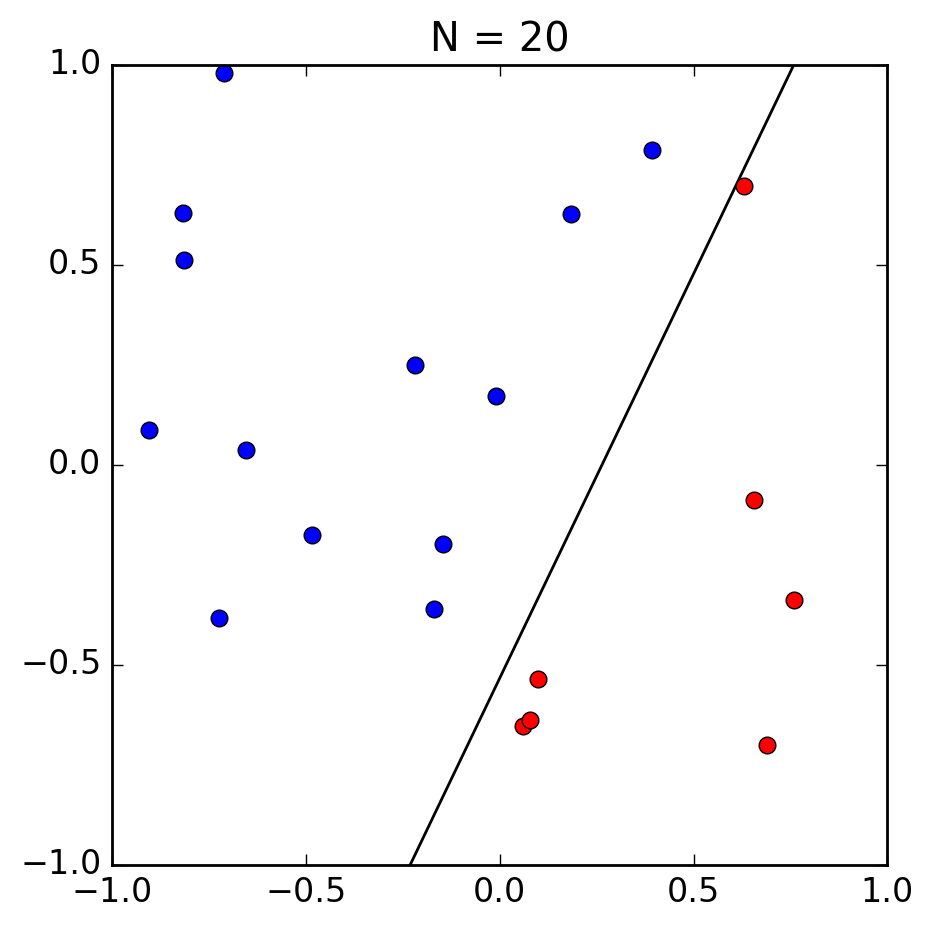
\includegraphics{14b.png}
	\caption{The final hypothesis $h(g)$ after 17 iterations.}
\end{figure}
\newpage

\subsection*{1.4c Run the Perceptron again with a data set size of 20 and compare results with 1.4b}

This time the Perceptron algorithm only required 14 iterations to find $h(g)$. The code was not modified at all for this section.

\begin{figure}[!htb]
	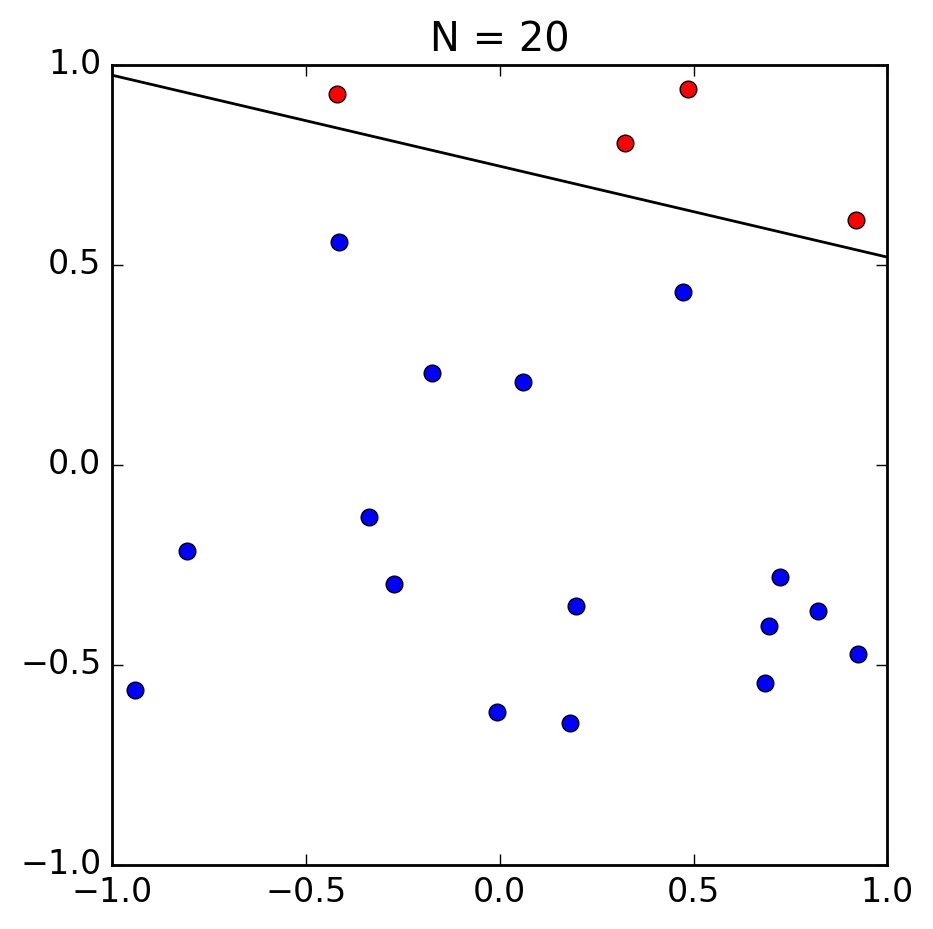
\includegraphics{14c.png}
	\caption{The final hypothesis h(g) after 14 iterations.}
\end{figure}
\newpage

\subsection*{1.4d Run the Perceptron again with a data set size of 100 and compare results.}

This time we ended up with 31 iterations and a much longer runtime to reach $h(g)$. It's looking like the runtimes get exponentially longer the more pieces of data introduced, as each entry may need to be re-checked for every iteration.

\begin{lstlisting}[frame=single]
p = Perceptron(100)
p.pla(save=True)
p.plot()
\end{lstlisting}

\begin{figure}[!htb]
	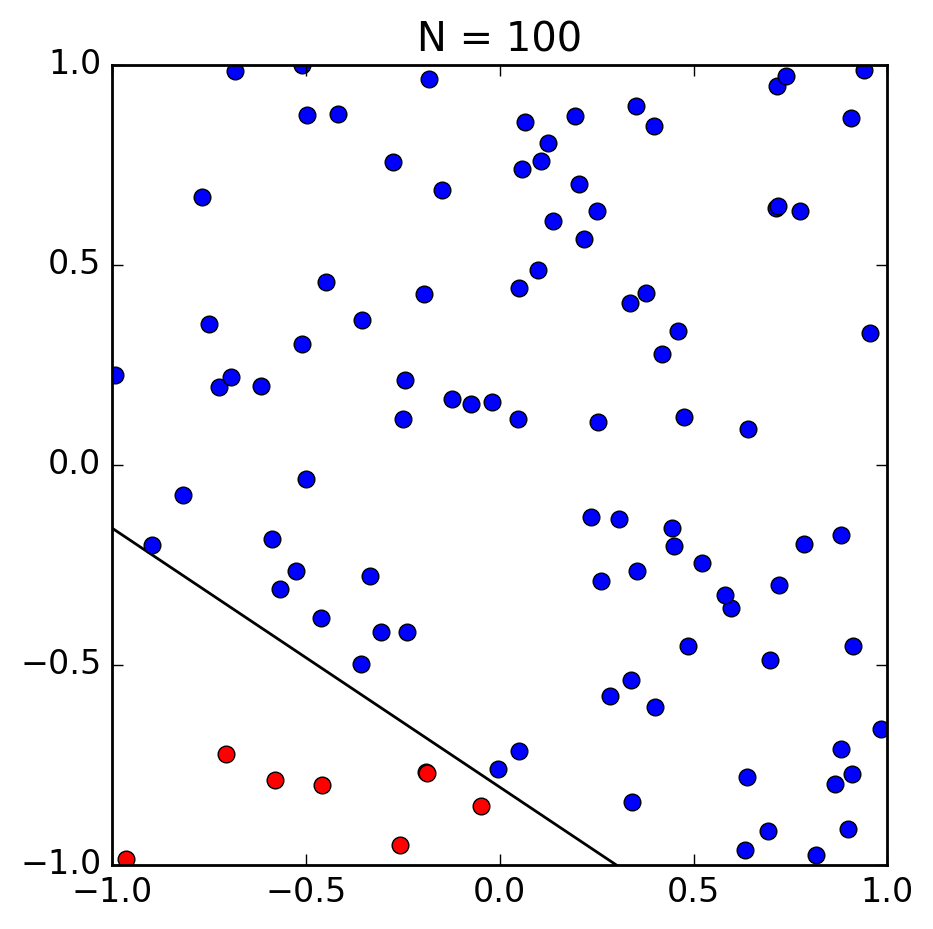
\includegraphics{14d.png}
	\caption{The final hypothesis $h(g)$ after 31 iterations.}
\end{figure}
\newpage

\subsection*{1.4e Run the Perceptron again with data set size of 1000. Compare results}

This section actually managed to freeze my computer after it had arrived at $h(g)$. It only required 49 iterations, but the runtime was significantly longer than any of the other experiments.

\begin{lstlisting}[frame=single]
p = Perceptron(1000)
p.pla(save=True)
p.plot()
\end{lstlisting}

\begin{figure}[!htb]
	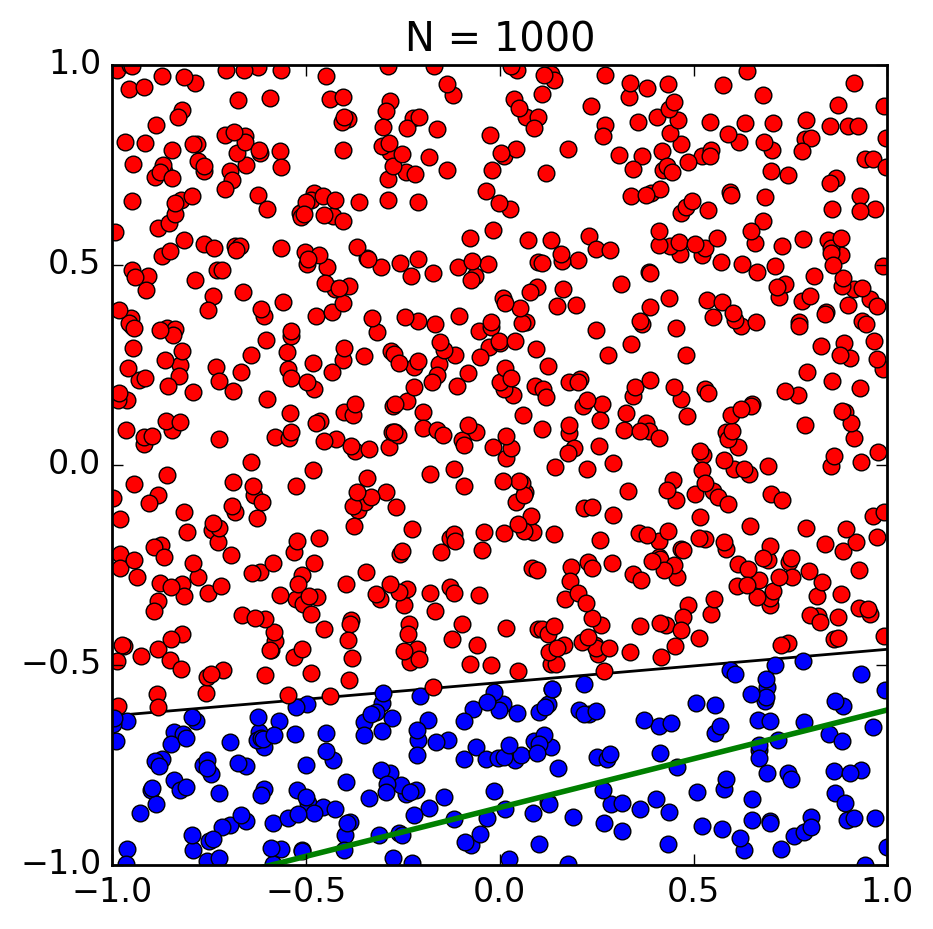
\includegraphics{14e.png}
	\caption{The final hypothesis $h(g)$ after 49 iterations.}
\end{figure}

However, after running the Perceptron a second time without saving the plots, it ran for 44052 iterations, so it seems I just got lucky with the first run.

\subsection*{1.4f Modify the algorithm to run in 10 dimensions rather than 2 and run the algorithm on a data set size of 1,000}

For this problem, the algorithm only took 1830 iterations to converge.
\newpage

\subsection*{1.4g Run the same algorithm as f 100 times, plot a histogram for the number of iterations taken to converge.}

To run the algorithm for this problem I added the following:

\begin{lstlisting}[frame=single]
for x in range(0, 100):
	p = Perceptron(1000)
	p.pla(save=False)

p = Perceptron(1000)
plt.hist(iterations)
plt.title("10th Dimension Perceptron Iterations")
plt.xlabel("Value")
plt.ylabel("Frequency")

fig = plt.gcf()

plot_url = py.plot_mpl(fig, filename='Iterations')
\end{lstlisting}

I used an array called iterations to store the number of iterations each run of pla needed to converge, and then turned the array into a histogram using plotly.

\begin{figure}[!htb]
	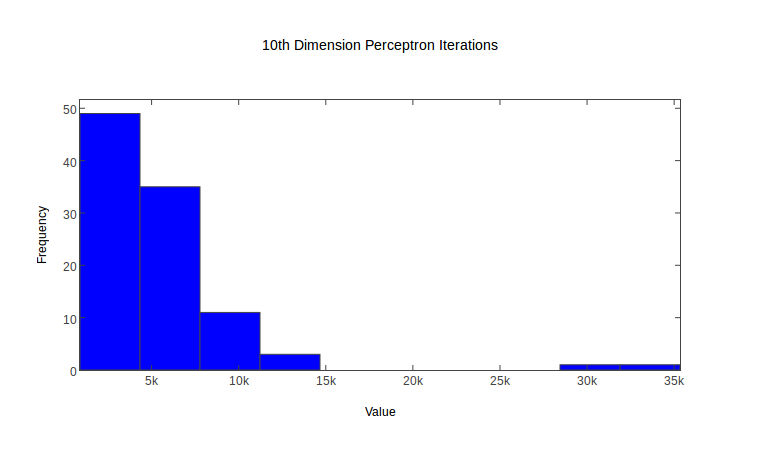
\includegraphics[scale=0.75]{Iterations.png}
	\caption{Histogram for problem 1.4g}
\end{figure}
\newpage

\subsection*{1.4h Summarize your conclusions with respect to accuracy and running time as a function of $N$ and $d$.}

I'm really not sure how to word this as a mathematical function, but it seems that as $N$ gets larger, the accuracy and runtime rise in accordance. The more data points introduced, the more iterations were necessary, but ultimately the hypothesis produced seemed to leave less room for error. Meanwhile by introducing more dimensions, we lessen our runtime by providing more possible "correct" answers that may leave a massively larger room for error, given that we are now extended into 10 dimensions rather than 2.

\end{document}